\section{Related Work}
\subsection{LLM-Assisted Hardware Design}
LLMs have been applied to hardware design at both the register-transfer level (RTL) and higher levels of abstraction. GPT4AIGChip uses LLMs to automate AI accelerator design \cite{10323953}, while Chip-Chat explores conversational interaction between an LLM and a human designer during microprocessor development \cite{10299874}. AutoChip and VeriGen generate and refine Verilog through iterative feedback and domain-specific adaptation \cite{thakur2024autochipautomatinghdlgeneration, 10.1145/3643681}. RTLCoder further improves open-source RTL generation through a specialized training dataset and model \cite{10720939}. Together, these studies demonstrate the potential of LLMs for architecture exploration, HDL generation, and iterative design repair.

High-level synthesis (HLS) provides another route for LLM-assisted hardware generation by leveraging the stronger code-generation capabilities of LLMs for C/C++. Prior work has shown that LLMs can refactor software-oriented C/C++ into synthesizable HLS implementations and assist design space exploration \cite{10691856}. HLSPilot automates HLS code generation and optimization through LLM-guided strategy selection \cite{xiong2024hlspilot}, while retrieval-augmented methods improve C-to-HLS conversion by supplying relevant design knowledge and examples \cite{10.1145/3670474.3685953}.

These approaches primarily optimize individual modules or accelerators. They do not address the system-level decisions required to transform a complete application into a customized SoC, including hotspot identification, hardware/software partitioning, accelerator generation and integration, and joint processor--accelerator optimization. SoCPilot builds on the code-generation and HLS capabilities of LLMs but applies them within an end-to-end, application-driven SoC design flow.
 
\subsection{SoC Design Automation}
Generator-based frameworks have substantially improved the modularity and reuse of SoC designs. Chisel provides a software-inspired hardware construction language for developing reusable and parameterized generators \cite{Chisel}. Rocket Chip builds on this abstraction to generate configurable RISC-V processors, caches, interconnects, and peripheral subsystems \cite{Asanovic:EECS-2016-17}. Chipyard integrates these generators with simulation, verification, and implementation tools, providing an extensible environment for full-system SoC exploration \cite{amid2020chipyard}.

Other platforms focus on heterogeneous integration and design space exploration. ESP provides a tile-based methodology for integrating RTL- and HLS-based accelerators, generating hardware/software interfaces, and prototyping complete systems on FPGAs \cite{mantovani2020agile}. ESP4ML specializes this flow for machine-learning accelerators \cite{esp4ml}, while ChipFlow supports hardware/software co-design for custom FPGA and ASIC systems \cite{chipflow2023}. MasterRTL accelerates early-stage architectural exploration using fast power, performance, and area estimation \cite{10577671}. Although these frameworks automate substantial portions of SoC construction, they generally require designers to specify the target architecture, select hardware components, and develop customized accelerators to be integrated.

Recent work has introduced LLM agents into SoC-level automation. 
SoCDev formulates SoC construction as a multi-agent TCL code-generation 
workflow for the Vivado Design Suite \cite{socdev2025}. 
GenSoC employs multiple agents to construct open-source IP libraries and 
automate IP selection, integration, and verification \cite{gensoc2025}. 
These methods demonstrate that LLM agents can coordinate tool execution 
and system integration beyond individual RTL modules, but primarily focus 
on project construction or reusable-IP composition.

Application-driven hardware/software co-design has also begun to leverage 
LLMs. Liao et al.~\cite{LiaoAL26} analyze the FALCON application using 
runtime profiling and LLM-based source analysis to identify acceleration 
candidates, and compare LLM-generated RTL accelerators with conventional 
HLS implementations on FPGA. This work demonstrates the potential of LLMs 
for application-level hotspot analysis and accelerator generation, but its 
evaluation primarily focuses on a small set of individual compute kernels 
rather than automated heterogeneous SoC construction and system-level 
optimization.

Table~\ref{tab:related_frameworks} summarizes the scope of representative 
LLM-assisted hardware and SoC design frameworks. Existing approaches 
typically automate either application-to-accelerator generation or 
IP-to-SoC construction. In contrast, SoCPilot connects application analysis, 
quantitative hardware/software partitioning, customized accelerator 
generation, heterogeneous SoC construction, and system-level optimization 
within a unified end-to-end flow.

\begin{table*}[t]
    \centering
    \caption{Comparison with representative LLM-assisted hardware and SoC design frameworks.}
    \label{tab:related_frameworks}
    \renewcommand{\arraystretch}{1.18}
    \setlength{\tabcolsep}{7pt}
    \resizebox{0.97\textwidth}{!}{
    \begin{tabular}{lccccccc}
        \toprule
        \textbf{Framework} &
        \textbf{\begin{tabular}[c]{@{}c@{}}Application\\Driven\end{tabular}} &
        \textbf{\begin{tabular}[c]{@{}c@{}}Profiling /\\Kernel ID\end{tabular}} &
        \textbf{\begin{tabular}[c]{@{}c@{}}HW/SW\\Partition\end{tabular}} &
        \textbf{\begin{tabular}[c]{@{}c@{}}Accelerator\\Generation\end{tabular}} &
        \textbf{\begin{tabular}[c]{@{}c@{}}SoC\\Generation\end{tabular}} &
        \textbf{\begin{tabular}[c]{@{}c@{}}System-level\\DSE\end{tabular}} &
        \textbf{\begin{tabular}[c]{@{}c@{}}End-to-End\\Validation\end{tabular}} \\
        \midrule

        HLSPilot~\cite{xiong2024hlspilot}
        & \checkmark
        & \checkmark
        & $\triangle$
        & \checkmark
        & --
        & --
        & $\triangle$ \\

        GenSoC~\cite{gensoc2025}
        & --
        & --
        & --
        & --
        & \checkmark
        & --
        & \checkmark \\

        SoCDev~\cite{socdev2025}
        & --
        & --
        & --
        & --
        & \checkmark
        & --
        & $\triangle$ \\

        Liao et al.~\cite{LiaoAL26}
        & \checkmark
        & \checkmark
        & $\triangle$
        & \checkmark
        & --
        & --
        & $\triangle$ \\

        \textbf{SoCPilot}
        & \checkmark
        & \checkmark
        & \checkmark
        & \checkmark
        & \checkmark
        & \checkmark
        & \checkmark \\

        \bottomrule
    \end{tabular}
    }
    
    \vspace{0.3em}
    \begin{minipage}{0.97\textwidth}
    \footnotesize
    \textit{Notation:} 
    \checkmark~denotes explicit support; 
    $\triangle$ denotes partial support or a limited scope; 
    -- denotes functionality that is not addressed as a primary objective.
    \end{minipage}
\end{table*}



\subsection{Benchmarks for LLM-Based SoC Design}
Application benchmarks provide the workloads needed to evaluate customized architectures. S2CBench contains synthesizable SystemC designs for HLS research \cite{6807518}; SHOC provides kernels and applications for evaluating heterogeneous computing systems \cite{10.1145/1735688.1735702}; and MachSuite supplies accelerator-oriented kernels spanning diverse computation and memory-access patterns \cite{6983050}. These suites support quantitative evaluation of performance and hardware cost, but they assume that the design flow and tool orchestration are already available. They therefore do not directly measure whether an LLM agent can complete the multistage process required to construct a working SoC.

System-level benchmarks for LLM-assisted SoC design have recently begun to address this gap. SoCDevBench evaluates LLM-generated TCL workflows for Vivado using design pass rate, FPGA resource utilization, and tool feedback \cite{socdev2025}. SLDB targets heterogeneous SoC integration and configuration with ESP-compatible designs, extending evaluation beyond isolated RTL generation \cite{sldb2025}. HSCO-Bench broadens the scope to end-to-end hardware/software co-design, covering kernel identification, HLS accelerator generation, ESP-based integration, and FPGA deployment \cite{hscobench2026}.
\begin{figure*}[htp]
    \centering
    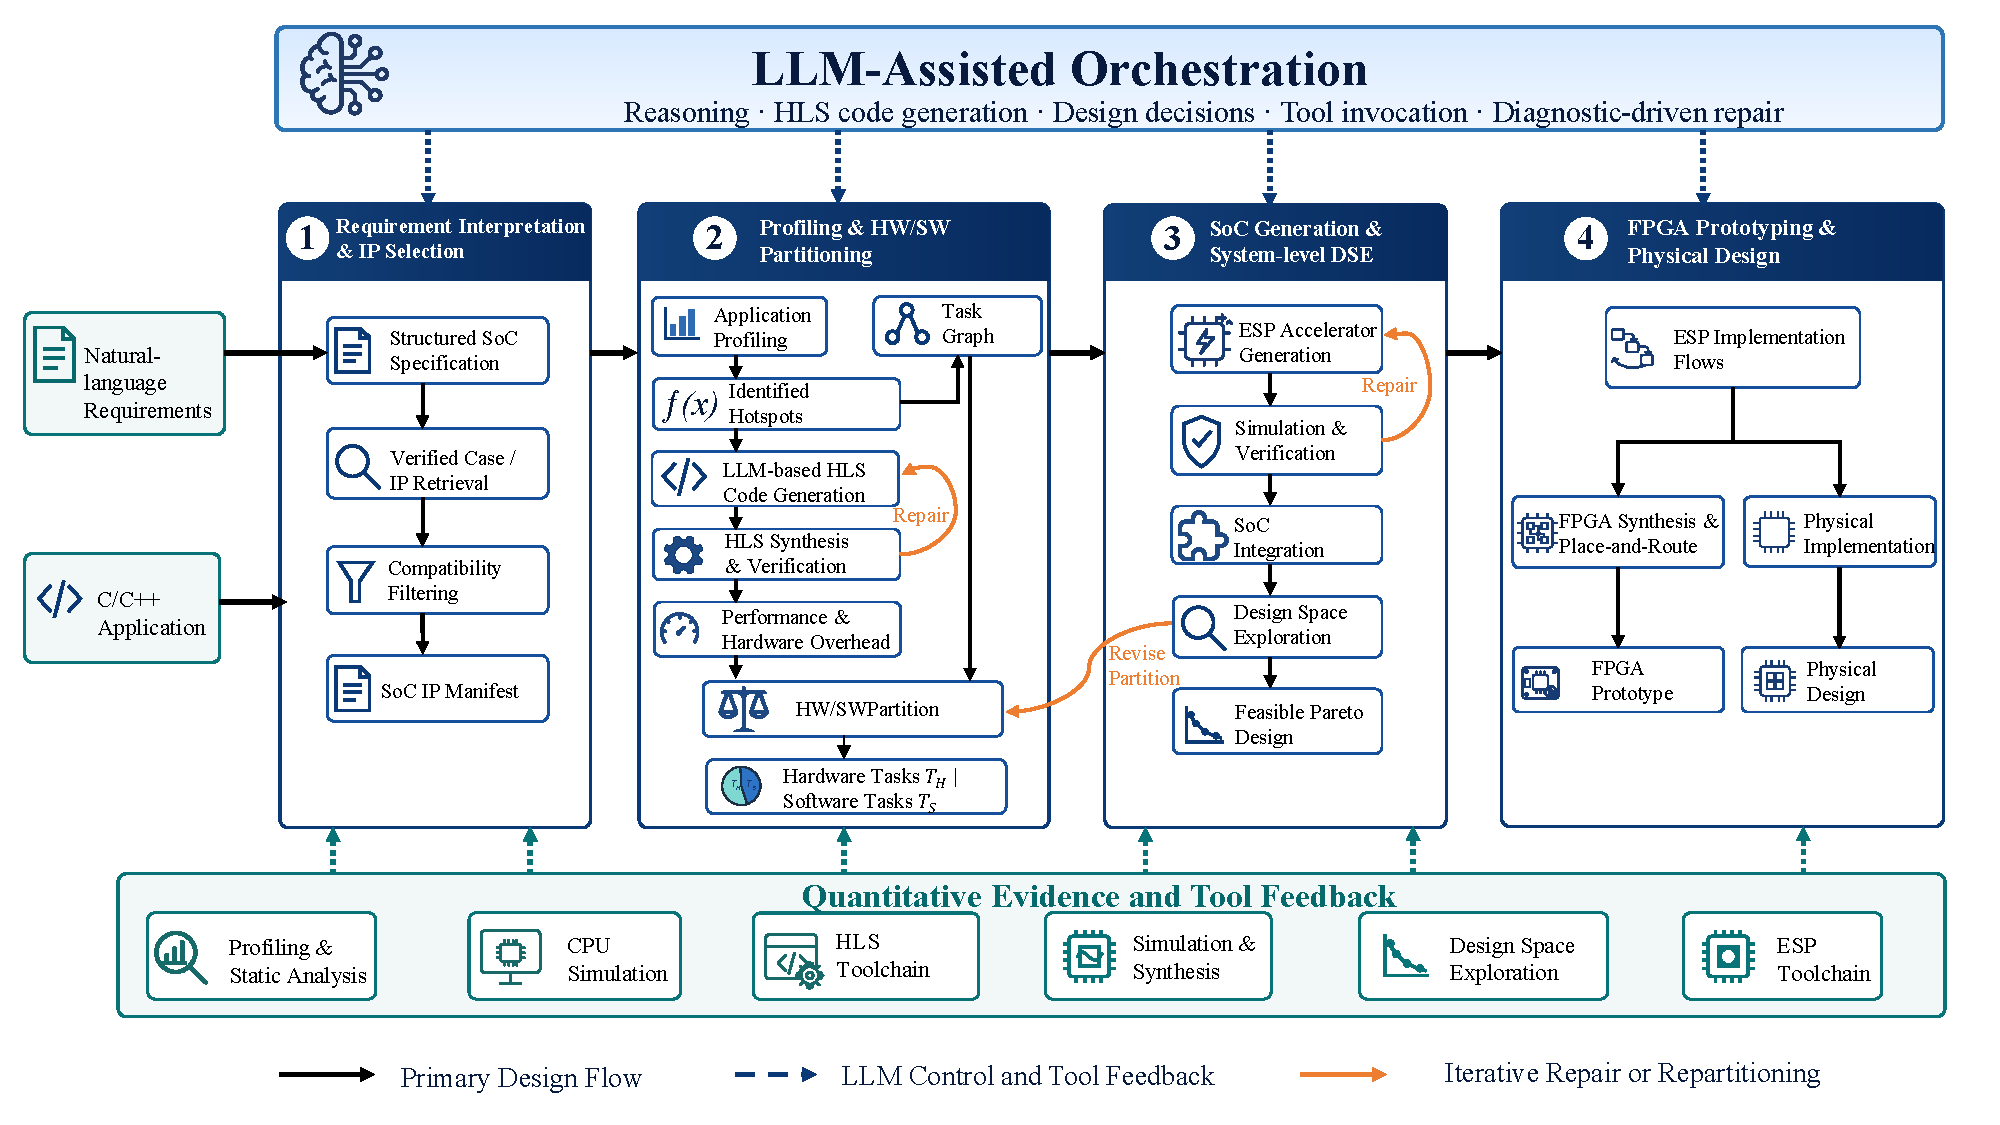
\includegraphics[width=0.98\textwidth]{pic/socpilot-framework.pdf} 
    \caption{Overview of the SoCPilot framework. SoCPilot uses an LLM orchestration layer and quantitative tool feedback to translate natural-language requirements and a C/C++ application into a customized SoC, covering requirement interpretation, HW/SW partitioning, accelerator and SoC generation, latency--area design space exploration, and FPGA prototyping and board validation. Embedded runtime software is manually prepared and is not generated by the LLM.}
\label{fig: overview}
    \vspace{-1em}
\end{figure*}
Together, these benchmarks reflect a progression from tool-script generation to heterogeneous integration and complete hardware/software co-design. They also show that system-level evaluation must consider not only code correctness, but also tool-flow completion, interface compatibility, hardware cost, and application-level performance. Complementing these task-oriented benchmarks, SoCPilot is evaluated on representative embedded applications and measures the complete workflow from hotspot discovery to FPGA-validated SoC generation and optimization.


